\documentclass[11pt]{scrartcl}
\usepackage{dominatrix}

% Graph Drawing Stuff
\usepackage{colortbl}
\usepackage{pgfplots}
\usepackage{tikz}
\usetikzlibrary{trees}
\usetikzlibrary{calc}
\pgfplotsset{compat=1.9}

% Tables
\usepackage{multirow}

% Strikeout
\usepackage{ulem}

% Jon's Name
\newcommand{\jon}{J\'{o}n }

% Additional Definitions
\newcommand{\og}{\ensuremath{\tilde{Y}}}
\newcommand{\eqname}[1]{\tag*{#1}}% Tag equation with name
\newcommand{\oneth}{\ensuremath{\alpha}}
\newcommand{\twoth}{\ensuremath{1-\alpha}}
\newcommand{\ve}{\varepsilon}

\title{Final Sample Test Answers}
\subject{ECON W3213 Spring 2014 \jon Steinsson}
\author{Linan Qiu, lq2137}

\begin{document}

\maketitle

\begin{abstract}
I made this set of answers in a rush (since I have 5 finals next week) and they may not be entirely correct. However, it may serve as an useful guide for you.
\end{abstract}

\section{True False Questions}

\subsection{Fiscal Multiplier}

True. On the Zero Lower Bound, the MP curve changes to a different one that slopes down, causing a larger than proportionate change in output gap. Check recitation notes or lecture notes for equations. This is very straightforward.

\subsection{Consumption}

False. Consumption expenditure does not track income. Should be smoothened. Again, provide necessary equations from lecture notes or recitation notes. They're all there.

\subsection{Friedman/Phelps Expectations Augmented Phillips Curve}

True. Under adaptive expectations, the Phillips curve shifts up and down entirely whenever there is positive or negative output gap respectively (hence below NAIRU unemployment or above). Hence, in the long run, the inverse relationship of the Phillips Curve doesn't hold. In the short run, it does.

\subsection{Fisher Equation}

Fisher equation with adaptive expectations says

\[ R_t = i_t - \mathrm{E}_t \pi_{t+1} = i_t - \pi_t \] 

If people expect deflation, $\mathrm{E}_t \pi_{t+1} < 0$. Then, with $i_t \approx 0$, $R_t < 0$

\subsection{Natural Experiments}

Uncertain. You can find the justifications on both sides in the last lecture for Fiscal Policy.

\section{Solow Model}

\subsection{Steady State Value for Capital}

At the steady state, where $K$ doesn't grow, hence $K_{t+1} = K_t$, 

\begin{align*}
s\bar{A}K^{\oneth}\bar{L}^{\twoth} &= dK_t \\
K_t^{\twoth} &= \frac{s\bar{A}\bar{L}^{\twoth}}{d} \\
K_t &= \left(\frac{s\bar{A}}{d}\right)^{\frac{1}{1-\alpha}}\bar{L}
\end{align*}

Hence steady state capital $\bar{K} = \left(\frac{s\bar{A}}{d}\right)^{\frac{1}{1-\alpha}}\bar{L}$

\subsection{Steady State Value for Output}

Simply substitute this expression for $\bar{K}$ into the output equation

\[\bar{Y} = \bar{A}\bar{K}^\alpha \bar{L}^{1-\alpha} \]

\subsection{Increase in Technology Level}

I explained this in my recitation notes, and I will just copy paste that section over (where I explained general changes in exogenous variables) and because I really don't have time to retype all of this.

Now assume that we were originally at $K = 500$, the steady state. Then, technology increased because we discovered penicillin. We can say that

\[A_1 = cA_0\] 

where $c$ is a constant greater than 1 that shows we've grown in terms of technology.

Then,

\[Y_t = cA_0K_t^\oneth L_t^\twoth \]

\[I_t = csA_0K_t^\oneth L_t^\twoth\]

\[C_t =  c(1-s)A_0K_t^\oneth L_t^\twoth\]

\[dK_t = dK_t\] 

Depreciation simply stays the same. 

We find that we arrive at a new steady state

\[\bar{K_0} = c^{\frac{1}{1-\alpha}}\left(\frac{s\bar{A}}{d}\right)^{\frac{1}{1-\alpha}}L \]

\begin{figure}[H]
\centering
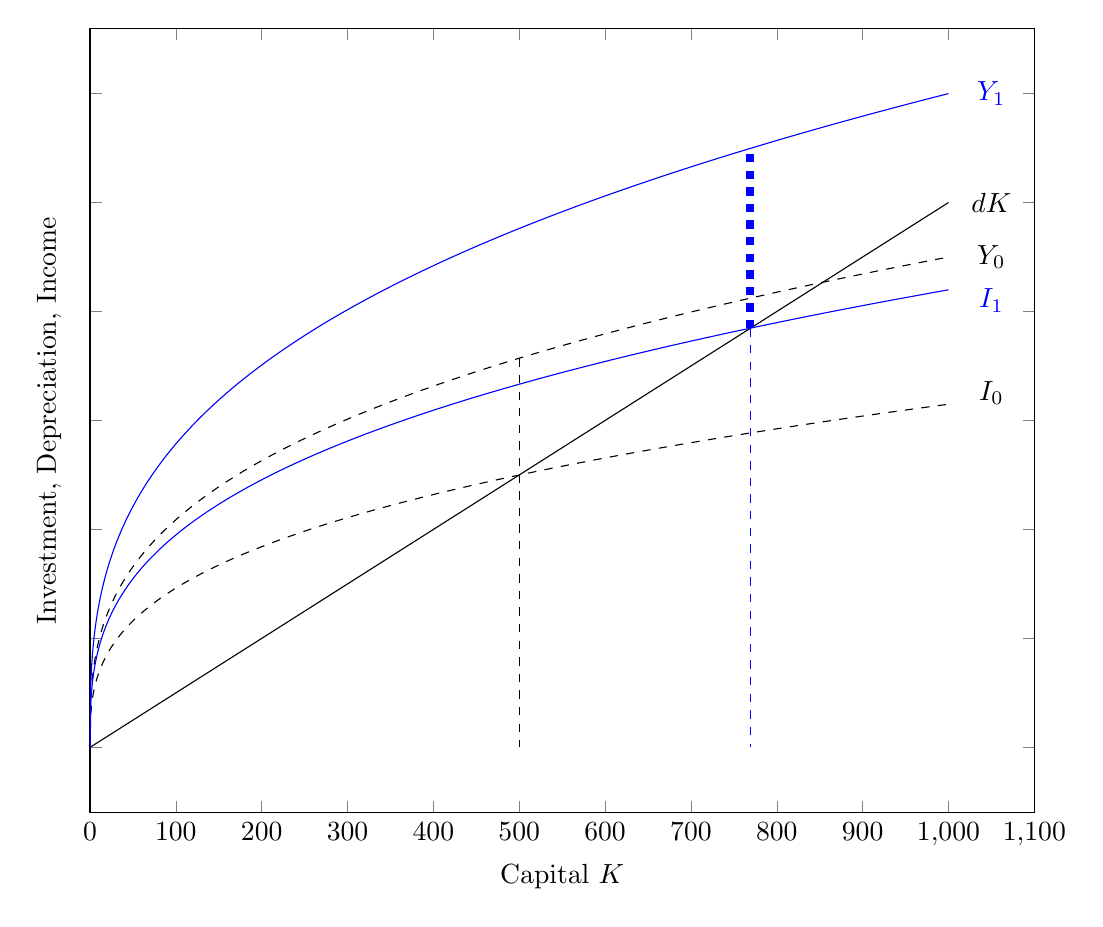
\begin{tikzpicture}
\begin{axis}[ylabel = {Investment, Depreciation, Income}, xlabel={Capital $K$}, yticklabels={,,},scale=1.75, xmin=0]
\addplot[domain=0:1000,black]
{x} node at (axis cs: 1050,1000) {$dK$};
\addplot[domain=0:1000,black,samples=1000, dashed]
{62.99*x^(1/3)} node at (axis cs: 1050,650) {$I_0$};
\addplot[domain=0:1000,black,samples=1000, dashed]
{90*x^(1/3)} node at (axis cs: 1050,900) {$Y_0$};

\addplot[domain=0:1000,black,samples=1000, blue]
{(62.99/90)*120*x^(1/3)} node at (axis cs: 1050,820) {$I_1$};
\addplot[domain=0:1000,black,samples=1000, blue]
{120*x^(1/3)} node at (axis cs: 1050,1200) {$Y_1$};

\addplot[domain=0:1000,black,dashed]
coordinates{(500,714) (500,0)};

\addplot[domain=0:1000,blue,dashed]
coordinates{(769,769) (769,0)};

\addplot[domain=0:1000,blue,dashed,line width=3]
coordinates{(769,769) (769,1100)};

\end{axis}
\end{tikzpicture}
\caption{Plot of investment, depreciation and income with capital $K$}
\end{figure}

Just as what we'd expect, we find that

\begin{itemize}
\item We have a completely new income function
\item We have a completely new investment function
\item Depreciation function stays the same
\item Steady state capital is larger
\item Steady state consumption is larger
\end{itemize}

\subsection{Solow Diagram}

(The diagram above with explanation should suffice. Again, this is in your lecture notes and in my recitation notes)

What happens is that at the original steady state $K=500$, we find that it is no longer a steady state with the new investment function. In fact, there will be positive net investment as investment is larger than depreciation. We will have positive capital growth, and we will keep experiencing that until we arrive at the new steady state.

\section{Price Level}

Skipped, answers are in lecture notes. 

\section{Friedman/Phelps Phillips Curve}

Without adaptive expectations, Phillips Curve will just be static. Hence, in order to lower unemployment or increase unemployment (positive or negative output gap), we will suffer only moderate inflation or disinflation respectively. This hints at a high sacrifice ratio. 

With adaptive expectations however, the Phillips Curve will shift up or down whenever there is below NAIRU unemployment or above NAIRU unemployment. (explain with equations and diagrams). Then, this will mean that even a tiny drop in unemployment (increase in output gap) will cause insane amounts of inflation. Sacrifice ratio will be very small.

\subsection{Okun's Survey}

Does not support adaptive expectation. Explanation above.

\subsection{Volcker's Action}

Supports adaptive expectation. Explanation above.

\subsection{Sargent's Evidence}

Supports adaptive expectation. Explanation above.

This question requires you to draw diagrams / use some equations (eg. trace out the dynamics of inflation spiraling out of control should a positive output gap persist. I'm taking the easy way out. DON'T DO THIS DURING YOUR EXAM.)

\section{Punch Bowl}

The general explanation for this type of question goes like this:

\begin{figure}[H]
\begin{subfigure}[b]{0.5\textwidth}
\centering
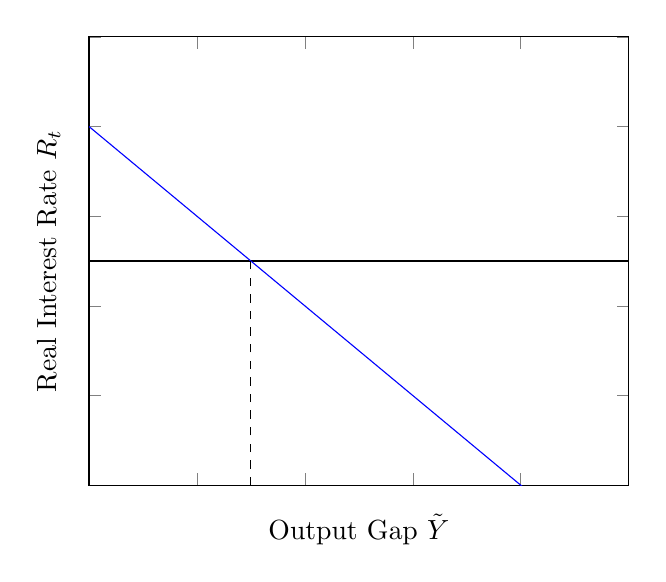
\begin{tikzpicture}
\begin{axis}[xlabel={Output Gap $\og$},ylabel={Real Interest Rate $R_t$},yticklabels={,,}, xticklabels={,,},ymin=0,ymax=10,xmin=0,xmax=10]
\addplot[black, domain=0:10]
{5};
\addplot[blue, domain=0:10]
{-x+8};
\addplot[black, domain=0:10, dashed]
coordinates{(3,0) (3,5)};
\end{axis}
\end{tikzpicture}
\caption{\color{blue}IS-\color{black}MP Diagram}
\end{subfigure}
\hspace{2ex}
\begin{subfigure}[b]{0.5\textwidth}
\centering
\begin{tikzpicture}
\begin{axis}[xlabel={Output Gap $\og$},ylabel={Inflation $\pi_t$},yticklabels={,,}, xticklabels={,,},ymin=0,ymax=10,xmin=0,xmax=10]
\addplot[black, domain=0:10]
{x};
\addplot[black, domain=0:10, dashed]
coordinates{(5,0) (5,5)};
\end{axis}
\end{tikzpicture}
\caption{Phillips Curve}
\end{subfigure}
\caption{Entire Economy}
\end{figure}

Now assume that we were originally at full employment. That's the point indicated by the dotted line.

What if we had an external shock that shifted the IS curve outwards? Then, IS shifts out. And we have a positive output gap. That will be reflected in the Phillips Curve too as we shift to a higher part of the same Phillips curve. That's what happens for this time period.

\begin{figure}[H]
\begin{subfigure}[b]{0.5\textwidth}
\centering
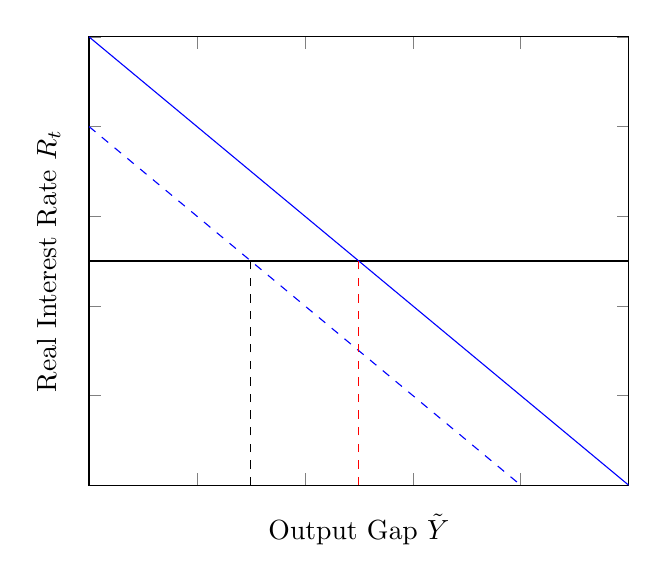
\begin{tikzpicture}
\begin{axis}[xlabel={Output Gap $\og$},ylabel={Real Interest Rate $R_t$},yticklabels={,,}, xticklabels={,,},ymin=0,ymax=10,xmin=0,xmax=10]
\addplot[black, domain=0:10]
{5};
\addplot[blue, domain=0:10, dashed]
{-x+8};
\addplot[blue, domain=0:10]
{-x+10};
\addplot[black, domain=0:10, dashed]
coordinates{(3,0) (3,5)};
\addplot[red, domain=0:10, dashed]
coordinates{(5,0) (5,5)};
\end{axis}
\end{tikzpicture}
\caption{\color{blue}IS-\color{black}MP Diagram}
\end{subfigure}
\hspace{2ex}
\begin{subfigure}[b]{0.5\textwidth}
\centering
\begin{tikzpicture}
\begin{axis}[xlabel={Output Gap $\og$},ylabel={Inflation $\pi_t$},yticklabels={,,}, xticklabels={,,},ymin=0,ymax=10,xmin=0,xmax=10]
\addplot[black, domain=0:10]
{x};
\addplot[black, domain=0:10, dashed]
coordinates{(5,0) (5,5)};
\addplot[red, domain=0:10, dashed]
coordinates{(7,0) (7,7)};
\end{axis}
\end{tikzpicture}
\caption{Phillips Curve}
\end{subfigure}
\caption{Entire Economy}
\end{figure}

Now our Phillips Curve doesn't stay constant in the next period. Nope, it shifts up because people are shmaaaaart. (or adaptive expectations. Professor Phelps please don't kill me for saying this)

\begin{figure}[H]
\begin{subfigure}[b]{0.5\textwidth}
\centering
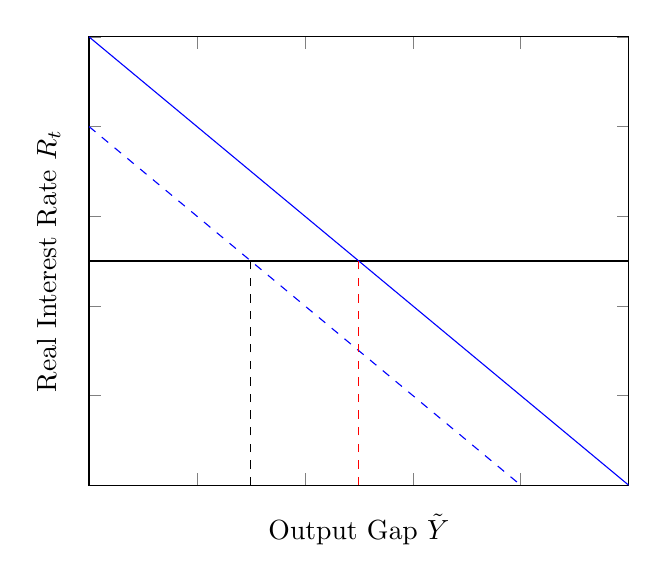
\begin{tikzpicture}
\begin{axis}[xlabel={Output Gap $\og$},ylabel={Real Interest Rate $R_t$},yticklabels={,,}, xticklabels={,,},ymin=0,ymax=10,xmin=0,xmax=10]
\addplot[black, domain=0:10]
{5};
\addplot[blue, domain=0:10, dashed]
{-x+8};
\addplot[blue, domain=0:10]
{-x+10};
\addplot[black, domain=0:10, dashed]
coordinates{(3,0) (3,5)};
\addplot[red, domain=0:10, dashed]
coordinates{(5,0) (5,5)};
\end{axis}
\end{tikzpicture}
\caption{\color{blue}IS-\color{black}MP Diagram}
\end{subfigure}
\hspace{2ex}
\begin{subfigure}[b]{0.5\textwidth}
\centering
\begin{tikzpicture}
\begin{axis}[xlabel={Output Gap $\og$},ylabel={Inflation $\pi_t$},yticklabels={,,}, xticklabels={,,},ymin=0,ymax=10,xmin=0,xmax=10]
\addplot[black, domain=0:10, dashed]
{x};
\addplot[black, domain=0:10]
{x+2};
\addplot[black, domain=0:10, dashed]
coordinates{(5,0) (5,5)};
\addplot[red, domain=0:10, dashed]
coordinates{(7,0) (7,9)};
\end{axis}
\end{tikzpicture}
\caption{Phillips Curve}
\end{subfigure}
\caption{Entire Economy}
\end{figure}

Now the central bank sees this and isn't happy. The inflation is gonna spiral out of control. So, it raises nominal interest rates, which increases real interest rates such that output gap goes back to the full employment level.

\begin{figure}[H]
\begin{subfigure}[b]{0.5\textwidth}
\centering
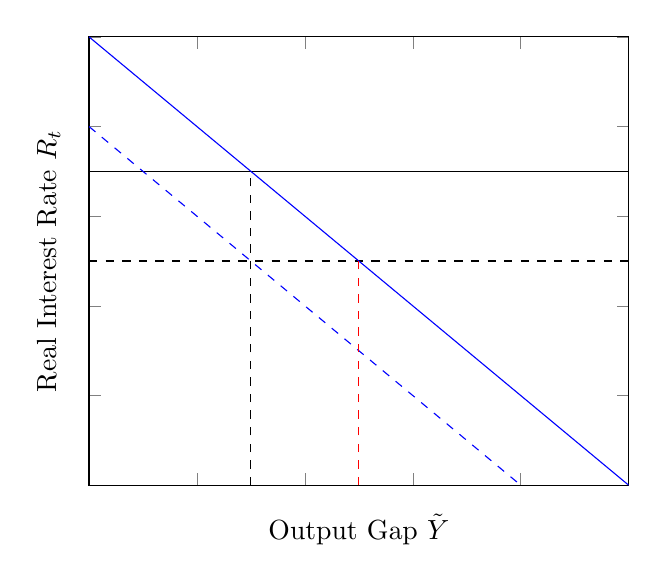
\begin{tikzpicture}
\begin{axis}[xlabel={Output Gap $\og$},ylabel={Real Interest Rate $R_t$},yticklabels={,,}, xticklabels={,,},ymin=0,ymax=10,xmin=0,xmax=10]
\addplot[black, domain=0:10, dashed]
{5};
\addplot[black, domain=0:10]
{7};
\addplot[blue, domain=0:10, dashed]
{-x+8};
\addplot[blue, domain=0:10]
{-x+10};
\addplot[black, domain=0:10, dashed]
coordinates{(3,0) (3,7)};
\addplot[red, domain=0:10, dashed]
coordinates{(5,0) (5,5)};
\end{axis}
\end{tikzpicture}
\caption{\color{blue}IS-\color{black}MP Diagram}
\end{subfigure}
\hspace{2ex}
\begin{subfigure}[b]{0.5\textwidth}
\centering
\begin{tikzpicture}
\begin{axis}[xlabel={Output Gap $\og$},ylabel={Inflation $\pi_t$},yticklabels={,,}, xticklabels={,,},ymin=0,ymax=10,xmin=0,xmax=10]
\addplot[black, domain=0:10, dashed]
{x};
\addplot[black, domain=0:10]
{x+2};
\addplot[black, domain=0:10, dashed]
coordinates{(5,0) (5,7)};
\addplot[red, domain=0:10, dashed]
coordinates{(7,0) (7,9)};
\end{axis}
\end{tikzpicture}
\caption{Phillips Curve}
\end{subfigure}
\caption{Entire Economy}
\end{figure}

Then, we first get zero output gap from our IS-MP diagram with a resulting higher real interest rate. Since we're at zero output gap, inflation stops spiraling out of control. We stay with a permanently higher inflation level. 

Your job in these two parts is then to identify the direction of the IS curve's initial shift. 

Personally, I interpret them as

\begin{enumerate}
\item Crazy optimism causes people to invest more. IS curve shifts outward.
\item Oil price shock causes people to spend less as everything becomes more expensive. IS curve shifts inward.
\end{enumerate}

So the explanation we did earlier explains the first case. For the second case where IS shifts left, just do the inverse.

\section{Innovation}

AHA. Told you market failure would be important! :P

I'm kidding.

\subsection{Motivates Government Intervention to Support Innovation}

Public goods. Explain non-excludable and non-rivalrous.

\subsection{Patent Protection and Inefficiencies}

Monopolies. Like Microsh*t.

\section{Glorious Revolution}

Explain the commitment problem using game theory. Draw beautiful trees. I have done them in my recitation notes. If you want, \jon did a really good explanation in the slides too.

\section{Spanish Unemployment}

\subsection{Current Position on IS-MP Diagram and Phillips Curve}

High unemployment, so there is a negative output gap. 

\begin{figure}[H]
\begin{subfigure}[b]{0.5\textwidth}
\centering
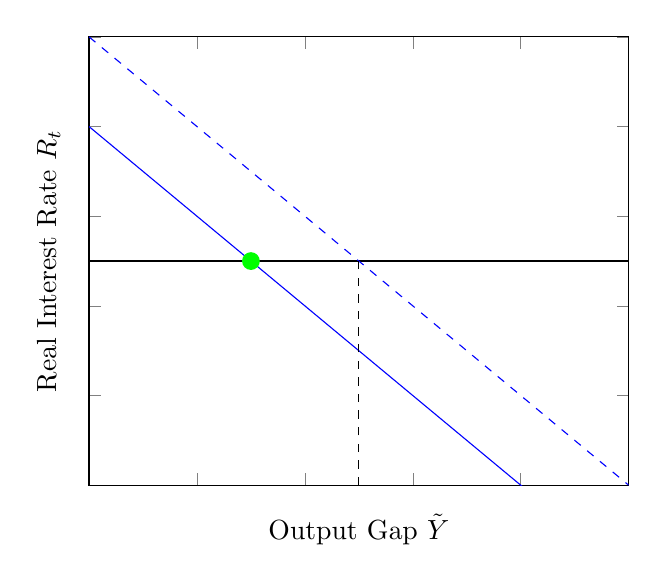
\begin{tikzpicture}
\begin{axis}[xlabel={Output Gap $\og$},ylabel={Real Interest Rate $R_t$},yticklabels={,,}, xticklabels={,,},ymin=0,ymax=10,xmin=0,xmax=10]
\addplot[black, domain=0:10]
{5};
\addplot[blue, domain=0:10]
{-x+8};
\addplot[blue, domain=0:10,dashed]
{-x+10};
\addplot[black, domain=0:10, dashed]
coordinates{(5,0) (5,5)};
\addplot[mark=*, green, mark size=3pt, domain=0:2]
coordinates{(3,5)};
\end{axis}
\end{tikzpicture}
\caption{\color{blue}IS-\color{black}MP Diagram}
\end{subfigure}
\hspace{2ex}
\begin{subfigure}[b]{0.5\textwidth}
\centering
\begin{tikzpicture}
\begin{axis}[xlabel={Output Gap $\og$},ylabel={Inflation $\pi_t$},yticklabels={,,}, xticklabels={,,},ymin=0,ymax=10,xmin=0,xmax=10]
\addplot[black, domain=0:10]
{x};
\addplot[black, domain=0:10, dashed]
coordinates{(5,0) (5,5)};
\addplot[mark=*, green, mark size=3pt, domain=0:2]
coordinates{(3,3)};
\end{axis}
\end{tikzpicture}
\caption{Phillips Curve}
\end{subfigure}
\caption{Entire Economy}
\end{figure}

The full employment line is indicated by the dashed black line. The green dot marks 'A'. On the left, the dashed blue line is what IS has to be if we were at full employment. The solid blue line is our current IS curve that's causing the output gap. On the Phillips Curve, we are at a point that's below the full employment line. 

\subsection{Autonomy over Monetary Policy}

If Spain had autonomy over its monetary policy, what it would do is to move its MP curve down until there is zero output gap. In other words, it should lower nominal interest rate $i_t$, and through the Fisher equation, influence Real Interest Rate $R_t$.

\[R_t = i_t - \pi_t\]

On the Phillips Curve, what that would do is to stop the Phillips Curve from shifting downwards (since we were originally at negative output gap, and that causes our Phillips Curve to keep moving down due to adaptive expectations). We will hence shift along the curve to a higher point. We arrive at zero output gap (since that's what the MP curve moved us to). 

\begin{figure}[H]
\begin{subfigure}[b]{0.5\textwidth}
\centering
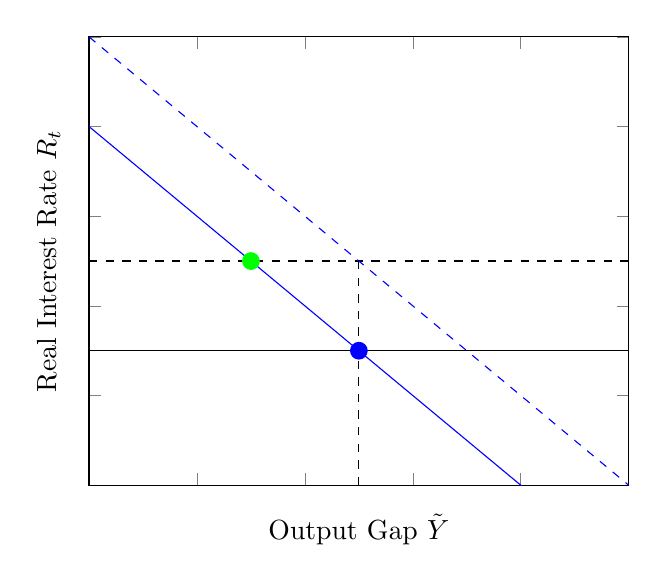
\begin{tikzpicture}
\begin{axis}[xlabel={Output Gap $\og$},ylabel={Real Interest Rate $R_t$},yticklabels={,,}, xticklabels={,,},ymin=0,ymax=10,xmin=0,xmax=10]
\addplot[black, domain=0:10, dashed]
{5};
\addplot[black, domain=0:10]
{3};
\addplot[blue, domain=0:10]
{-x+8};
\addplot[blue, domain=0:10,dashed]
{-x+10};
\addplot[black, domain=0:10, dashed]
coordinates{(5,0) (5,5)};
\addplot[mark=*, green, mark size=3pt, domain=0:2]
coordinates{(3,5)};
\addplot[mark=*, blue, mark size=3pt, domain=0:2]
coordinates{(5,3)};
\end{axis}
\end{tikzpicture}
\caption{\color{blue}IS-\color{black}MP Diagram}
\end{subfigure}
\hspace{2ex}
\begin{subfigure}[b]{0.5\textwidth}
\centering
\begin{tikzpicture}
\begin{axis}[xlabel={Output Gap $\og$},ylabel={Inflation $\pi_t$},yticklabels={,,}, xticklabels={,,},ymin=0,ymax=10,xmin=0,xmax=10]
\addplot[black, domain=0:10]
{x};
\addplot[black, domain=0:10, dashed]
coordinates{(5,0) (5,5)};
\addplot[mark=*, green, mark size=3pt, domain=0:2]
coordinates{(3,3)};
\addplot[mark=*, blue, mark size=3pt, domain=0:2]
coordinates{(5,5)};
\end{axis}
\end{tikzpicture}
\caption{Phillips Curve}
\end{subfigure}
\caption{Entire Economy}
\end{figure}

The dashed black line now represents the previous MP curve, and the solid black line the new MP curve due to the lowering of nominal interest rates (by increasing money supply). We then move to the Real Interest Rate indicated by the blue dot, together with output gap of zero. This shifts us along the Phillips Curve to a higher inflation level with zero output gap.

\subsection{No Autonomy over Monetary Policy}

In this case, since the rest of Europe is at full employment, there is no reason for the rest of the countries to demand loose monetary policy. Then, the MP curve will stay where it is.

In that case, since Spain is at a negative output gap, there will be disinflation due to adaptive expectation. To illustrate this, let's bring out the good ol' Phillips Curve.

\[ \pi_t = \pi_{t-1} + \bar{v} \og_t + \bar{o} \] 

Now we know that if $\og_t$ is negative, then the situation below happens. Assume that we start with $\og_t = -2$ (to represent the negative output gap and $\pi_{-1} = 0$. $\bar{v} = 1$ and $\bar{o} = 0$ for convenience.

Then,

\begin{align*}
\pi_0 &= 0 - 2 + 0 = -2 \\ 
\pi_1 &= -2 - 2 + 0 = -4 \\ 
\pi_2 &= -4 - 2 + 0 = -6
\end{align*}

In other words, so long as there is a negative $\og_t$ that persists, inflation will keep decreasing. This is the precisely due to people expecting disinflation and factoring that into their pricing.

Hence, Spain will experience disinflation (or inflation that is lower than the rest of Euro area) over the near future.

On a diagram, what will happen is that

\begin{figure}[H]
\begin{subfigure}[b]{0.5\textwidth}
\centering
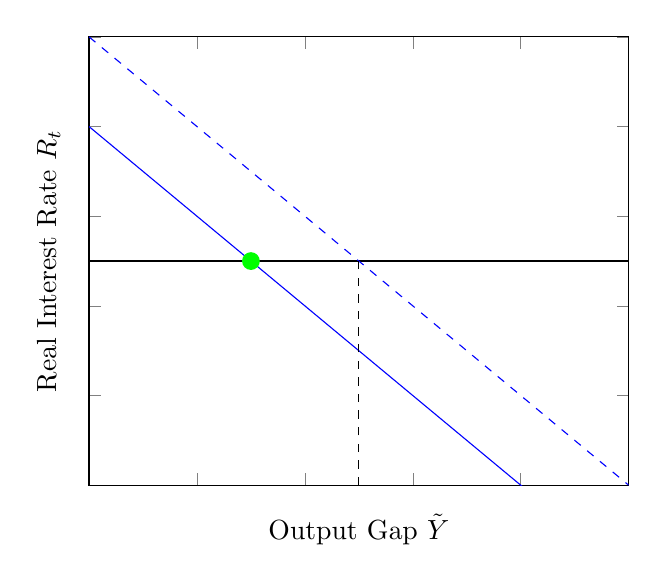
\begin{tikzpicture}
\begin{axis}[xlabel={Output Gap $\og$},ylabel={Real Interest Rate $R_t$},yticklabels={,,}, xticklabels={,,},ymin=0,ymax=10,xmin=0,xmax=10]
\addplot[black, domain=0:10]
{5};
\addplot[blue, domain=0:10]
{-x+8};
\addplot[blue, domain=0:10,dashed]
{-x+10};
\addplot[black, domain=0:10, dashed]
coordinates{(5,0) (5,5)};
\addplot[mark=*, green, mark size=3pt, domain=0:2]
coordinates{(3,5)};
\end{axis}
\end{tikzpicture}
\caption{\color{blue}IS-\color{black}MP Diagram}
\end{subfigure}
\hspace{2ex}
\begin{subfigure}[b]{0.5\textwidth}
\centering
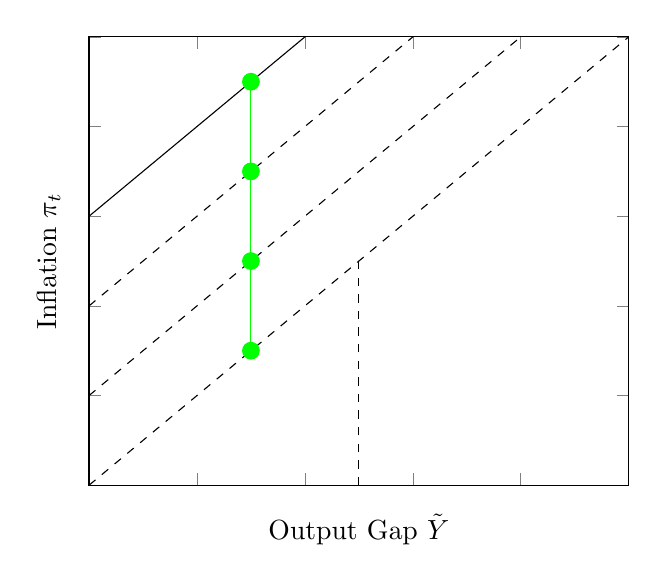
\begin{tikzpicture}
\begin{axis}[xlabel={Output Gap $\og$},ylabel={Inflation $\pi_t$},yticklabels={,,}, xticklabels={,,},ymin=0,ymax=10,xmin=0,xmax=10]
\addplot[black, domain=0:10,dashed]
{x};
\addplot[black, domain=0:10,dashed]
{x+2};
\addplot[black, domain=0:10,dashed]
{x+4};
\addplot[black, domain=0:10]
{x+6};
\addplot[black, domain=0:10, dashed]
coordinates{(5,0) (5,5)};
\addplot[mark=*, green, mark size=3pt, domain=0:2]
coordinates{(3,3) (3,5) (3,7) (3,9)};
\end{axis}
\end{tikzpicture}
\caption{Phillips Curve}
\end{subfigure}
\caption{Entire Economy}
\end{figure}

The Phillips Curve keeps moving up and we have inflation levels indicated by the green line and dot.

\end{document}